% Intended LaTeX compiler: pdflatex
\documentclass[a4paper, dvipdfmx, 10pt]{article}
\usepackage[utf8]{inputenc}
\usepackage[T1]{fontenc}
\usepackage{graphicx}
\usepackage{grffile}
\usepackage{longtable}
\usepackage{wrapfig}
\usepackage{rotating}
\usepackage[normalem]{ulem}
\usepackage{amsmath}
\usepackage{textcomp}
\usepackage{amssymb}
\usepackage{capt-of}
\usepackage{hyperref}
\usepackage{minted}
\usepackage{amsmath, amssymb, bm}
\usepackage{graphics}
\usepackage{color}
\usepackage{times}
\usepackage{longtable}
\usepackage{minted}
\usepackage{fancyvrb}
\usepackage{indentfirst}
\usepackage{pxjahyper}
\usepackage[utf8]{inputenc}
\usepackage[backend=biber, bibencoding=utf8]{biblatex}
\usepackage[top=20truemm, bottom=25truemm, left=25truemm, right=25truemm]{geometry}
\usepackage{ascmac}
\usepackage{algorithm}
\usepackage{algorithmic}
\addbibresource{/home/meguru/Github/private-Journal/research-plan/reference.bib}
\author{MokkeMeguru}
\date{}
\title{スケッチ to イラストな手法、style2paint を読む}
\hypersetup{
 pdfauthor={MokkeMeguru},
 pdftitle={スケッチ to イラストな手法、style2paint を読む},
 pdfkeywords={},
 pdfsubject={},
 pdfcreator={Emacs 26.2 (Org mode 9.2.3)}, 
 pdflang={Ja}}
\begin{document}

\maketitle
\section{導入}
\label{sec:org3193845}
\begin{figure}[htbp]
\centering
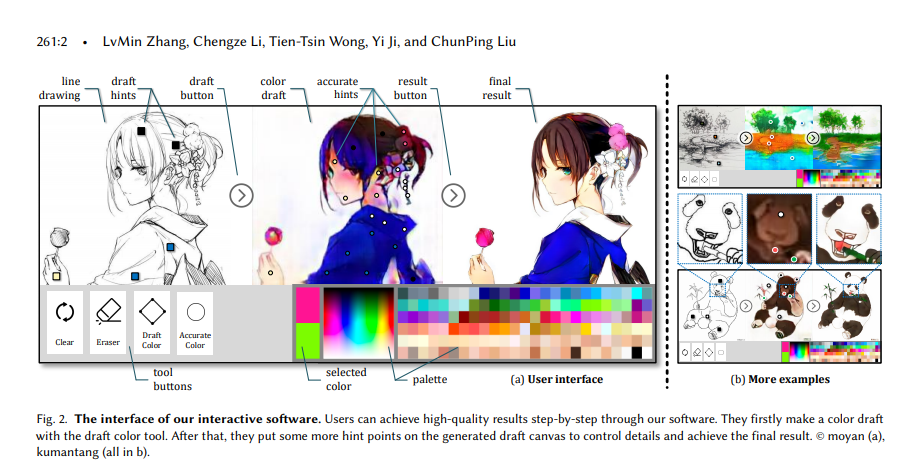
\includegraphics[width=.9\linewidth]{./img/style2paint_app.PNG}
\caption{style2paint 実アプリケーション図}
\end{figure}

\begin{quote}
良い感じのお絵描きの補助ツールが欲しい!(友人談)\\
\end{quote}

  最近ですと、ClipStudio Paint Pro/Ex が \textbf{自動着彩機能} を beta 版で利用可能になるなど、 \textbf{お絵描き支援に関する研究} が \textbf{市場価値} を生んでいますね。\\
( \sout{学術的にどうかって?医療データでもない深層学習にお金が下りると思ってんの?} )。\\

そんなわけでスケッチtoイラストみたいな研究論文が海外や国内企業ではそれなりに数が出ているわけなんですが、その中でも即プロダクトに活かせる程度に高度なものとして \href{https://github.com/lllyasviel/style2paints}{style2paint} というものがあります。これはラフ画からい感じに着彩するというまさに文脈通りの機能を実現するためのもので、実際に対話型のソフトウェアが構築されたものです。これはバージョンが存在しており、2019年6月時点で最新となっているのは v4 です。これに関する論文が、\href{https://github.com/lllyasviel/style2paints/blob/master/papers/sa.pdf}{Two-stage Sketch Colorization} というものです。\\

個人的な導入はともかくとして、簡単に論文で述べられている導入の方に踏み込んでみましょう。\\

\begin{quote}
着彩って難しくて時間かかるし、説得力のある絵を書くには、絵師でも苦労するよね。初心者の人にはお手本となるような、絵師さんには沢山の色の組み合わせを試せるような(例えば髪の色をちょっと変えてみたりとか)仕組みを作る必要があると思うんだ。\\

でも着彩にの自動化をしようと思ったら結構多くの課題があって、例えば主題(人とか猫とか)を制限していない状態でのスケッチ画をモデルに理解してもらうのは至難の業だし、スケッチ画は線画に比べれば大分抽象化されているからそこの差を埋めるようにしないといけない、質感とか陰影みたいな情報も描かれていないからそれの推測もしなくちゃぁいけない。\\

ところで最近だと深層学習の技術が発展してきて、\href{https://nico-opendata.jp/ja/casestudy/comicolorization/index.html}{Comicolorization} なんかの技術が便利な着彩補助の関連研究として出てきているね。でもこいつらはにじみとか色の間違いとかが普通にあったりするんだ。これらを修正できるようにしなきゃいけないんだけど、スケッチ -> 着彩の間に僕たちユーザは上手いこと手を出すことが出来ていなくて、結局自動着彩の技術よりも手打ちの着彩の方がまだまだ人気という感じなんだ。\\

そんなわけで僕たちは自動着彩じゃなくて半自動着彩のフレームワークを提案するよ。半自動というのはどういうことかっていうと、ユーザが着彩結果をちょいちょい弄って修正できるようにしているっていう意味、つまりスケッチ->着彩(1)->ユーザの修正->着彩(2)->\ldots{}->着彩(マスター) みたいなことをしたいってことだね。\\
提案したフレームワークは、2段階に別れたCNNベースのもので、一つ目は簡単に色をちらして色の概略図みたいなものを作るもの、もう一つはそこから間違いや変な質感になっているものなんかを修正して細かいところを詰めていくものになっているよ。繰り返しになるかもしれないけど、つまりスケッチ -> 着彩という問題をより単純な2つのタスクに分離したってことだね。これによってモデルの学習が効率化して、そのモデルが堅牢なものになったことがわかったよ。更に言うと、既存の着彩補助に関する手法で得られた着彩画を修正することもできることがわかったんだ。\\

それで現実世界でうまく適用できるか試すためにGUIアプリを作ってユーザに使ってもらったんだけど、この手法は2段階に分かれているとはいえ、ユーザが途中結果を見ながら修正ができることなんかも相まって、ユーザからの満足度は高かったよ。\\

評価として用いた手法が、実アプリケーションを用いたユーザアンケートだよ。これによって既存手法より良いということを示しています。\\

最後に簡単に僕達が出来たことをまとめるとこんな感じになるよ。\\

\begin{enumerate}
\item 実世界で作られているスケッチから高品質な着彩ができる2段階の着彩モデルを作ったよ\\
\item 僕たちの提案した手法は、既存の手法と比較して着彩の誤り修正が容易でより高品質な着彩結果を得ることができるようになったよ\\
\item 実際にユーザに使ってもらえるように、実アプリケーションを作ってみたよ\\
\end{enumerate}
\end{quote}

ほぼほぼ全意訳ですが、導入でおおよそ重要なことを述べきっている論文なのでもりもり書いています。\\


\section{関連研究}
\label{sec:org2fced56}
沢山ありましたので、公開されているものか、読んでみて面白そうだったものか、実際に試して面白かったものだけを抜粋して簡潔に紹介します。\\

\subsection{色伝搬}
\label{sec:orgf5794f8}
スケッチ->単色で塗りつぶし\\

\begin{itemize}
\item \href{https://dcgi.fel.cvut.cz/home/sykorad/Sykora09-EG.pdf}{Lazy Brush}\\

スケッチからいい感じに領域選択して色を塗りつぶす研究。深層学習とかの手法でもないし、恐らく機械学習というわけでもないです。\href{http://animatetvp.blogspot.com/2015/01/lazybrush.html}{実アプリケーションとしてある}らしく、チュートリアルムービーを見ることが出来ますが、めっちゃ早いです。領域選択系になるので、医療データの癌領域特定なんかに活かせそうですね。大学かなんかでやればいいんじゃないっすかね。\\
\end{itemize}

\subsection{機械学習ベースの自動着彩}
\label{sec:orgf10d670}
スケッチ->カラー画像 or グレースケール画像->カラー画像\\
Scribbler はざっくり言うと、encoder-decoder型のGenerator+GANsのDiscriminatorのような形を取っています。この部分の研究だと、敵対性ネットワークを用いるのがデフォルトという感じになるようです。\\

\begin{itemize}
\item \href{https://arxiv.org/abs/1612.00835}{Scribbler}\\

スケッチ から カラー画像 or 線画+補助色 から カラー画像を作る手法です。要所要所に色の情報を付け加えることで、より良い画像が出来る、というもので、本手法にはそれなりに近いのかな、と思いました。但しスケッチのクオリティが高すぎるので、初心者のお絵描き補助という目的に沿うことができるようには思えない感じです。\\
\begin{figure}[htbp]
\centering
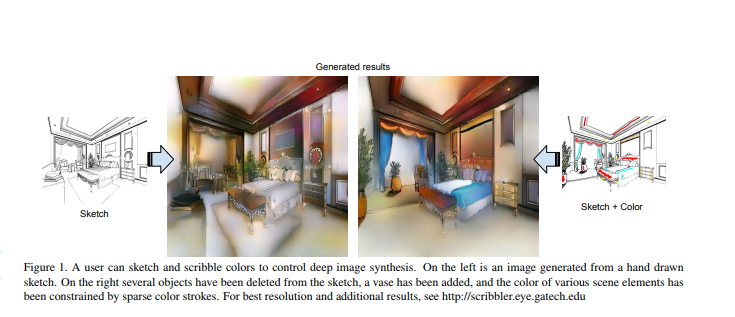
\includegraphics[width=.9\linewidth]{./img/scribbler_abst.png}
\caption{Scribbler より引用}
\end{figure}

\item \href{https://arxiv.org/pdf/1704.08834.pdf}{Outline Colorization through Tandem Adversarial Networks.}\\

グレースケールの画像 から カラー画像を作るための手法です。色彩予測を行うネットワークと、シェーディングを行うネットワークを組み合わせて画像を作り出すネットワークです。グレースケール画像から色の予測を行い、その色予測と、元のグレースケール画像の陰影情報を組み合わせて画像を作る、というモデル(学習にはGANsのDiscriminatorを使う)で style2paint とは違った2段階モデルになっています。\\

\item \href{https://arxiv.org/pdf/1705.01908.pdf}{AutoPainter}\\

スケッチ から カラー画像を作るための手法です。GANsを用いた自動着彩について研究したいなら一度は読みたい、という感じに読みやすい論文です。(というよりは損失関数の定義がすごくわかりやすい形にな収まっている。)pix2pix とのみ比較しているのでどの程度の性能なのかイマイチ理解が出来ないところがありますが、少なくとも pix2pix に対しては圧勝しています。\\

面白かったのでもう少し気になったところを書くと、損失関数に画像の滑らかさを付け足す項を追加している点で、それは以下のような式になります。\\

\(L_{tv} = \sqrt{(y_{i+1, j} - y_{i, j})^2 + (y_{i, j+1} - y_{i, j})^2 }\)\\

この式は他の画像生成系の論文ではあんまり見ないものだったので(というよりくっきりした画像を作るのがGANsのVAEに対する強みの一つなので、それを潰しているようにも捉えられるということが不思議です)、面白みがあるなぁと思いました。\\

ちなみに一時期 PaintChainer の論文の盗作なのでは?という議論が上がったりもしていましたが、これは恐らく間違いです。\\

\item PaintsChainer シリーズ\\

スケッチ->カラー画像を作るための手法です。PFN の出した \href{https://paintschainer.preferred.tech/index\_ja.html}{つよつよ成果物} を引っさげたシリーズです。名前が、たんぽぽ->かな->さつき、となっている \texttt{舐め腐った} 特徴的なタイトルのものです。\href{https://github.com/pfnet/PaintsChainer/issues/146}{論文}がないっぽいんですが、これはどういうこっちゃ…?\\

\item \href{https://arxiv.org/abs/1706.06918}{cGAN-based Manga Colorization Using a Single Training Image}\\

グレースケール漫画 から カラー漫画を作るための手法です。物凄い面白い手法を使っているんですが、簡単な特徴に関する説明は \href{http://yusuke-ujitoko.hatenablog.com/entry/2017/07/01/234633}{このページ} にあります。大量のデータで殴りつける最近のビッグデータでグローバルなジャパニーズドリーム()なものとは違い、とても日本人臭い泥にまみれた手法を使っているので、一度読んでみると面白いと思います。\\

ちなみにこの手法を用いて低賃金で鬼のように働かされている日本人の漫画家やアニメータを救おう!みたいな \href{http://broncoscholar.library.cpp.edu/bitstream/handle/10211.3/207996/YanYiyang\_Thesis2018.pdf?sequence=3}{調査論文} が \textbf{海外} で出ているのは、これも日本らしくて大好きです。\\
\end{itemize}

\subsection{画像のスタイル変換}
\label{sec:org39b8f80}
画像のスタイル変換もスケッチ->カラー画像に使えるので関連研究として取り上げられています。\\

\begin{itemize}
\item \href{https://arxiv.org/abs/1711.09554}{Discriminative Region Proposal Adversarial Networks for High-Quality Image-to-Image Translation}\\

GANsを用いた画像のスタイル変換に関する論文。教師あり学習。例えばセグメンテーション画像(オブジェクトごとに色分けされた画像…?)と写真のような画像との変換、線画から写真のような画像の変換、あるいはそれらの逆元が出来る、と主張されています。実装は \href{https://github.com/godisboy/DRPAN}{こちら} から。DRPAN という GANs の応用みたいなモデルを使っているんですが、僕の低脳では理解できませんでした…\\

\begin{figure}[htbp]
\centering
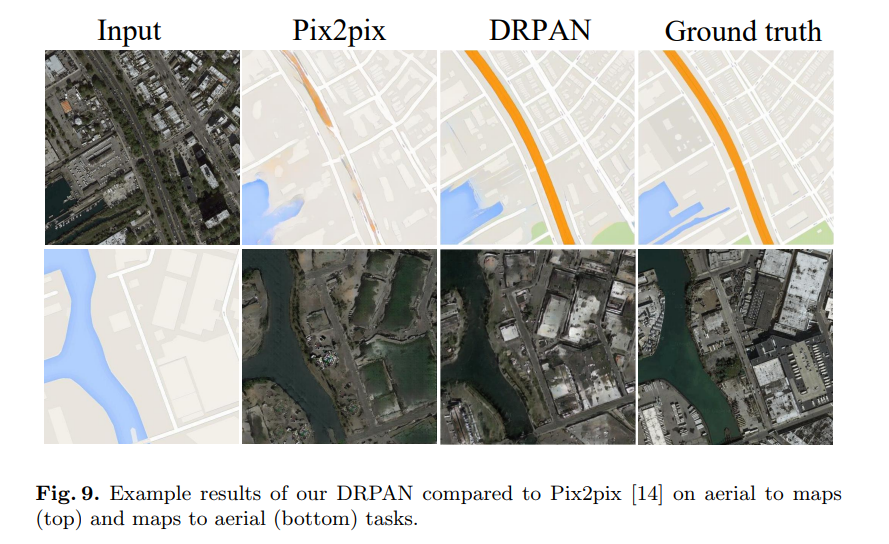
\includegraphics[width=.9\linewidth]{./img/drp_abst.PNG}
\caption{論文より引用}
\end{figure}

\item \href{https://arxiv.org/abs/1605.09782}{Adversarial Feature Learning}\\

教師なし学習。これはスタイル変換という文脈ではなく、双方向 GANs を求める研究であることに注目しました。最近ですと Flow-base のモデルが可逆な潜在表現獲得モデルとして有名ですが、GANsでもそのような試みが行われているという意味で非常に興味深かったです。GANs に関する数式がもりもりしているので、GANs の数式をたくさん見てみたい人なんかも読んでみると楽しいかもしれません。というかこの論文が読めれば GANs マスターってくらいには GANs を理解できると思います。\\

\item \href{https://arxiv.org/pdf/1703.00848.pdf}{Unsupervised Image-to-Image Translation Networks}\\

教師なし学習。実装は \href{https://github.com/mingyuliutw/unit}{こちら} 。ドメインを2つ仮定して、それぞれのドメインにおける同義の意味を同じ潜在表現として取り扱うことでスタイル変換を行おうとしています。つまり \(X_1\) のドメインからある画像 a と \(X_2\) のドメインから a と同じシチュエーションなある画像 b について考えたときに、それぞれの潜在表現は同じ z ということになります。Generator や Discriminator はスタイルごとに必要になります。つまり \(X_1\) のスタイルの画像についての Discriminator は、 \(X_1\) から得られる画像か、 \(X_2\) から得られた画像の潜在表現から \(G_1\) を通して得られた \(X_1\) のスタイルになった画像を判定するものになります。この論文をチョイスした理由は、自然言語含めスタイル変換全般に使えそうな手法だったからです。あとこれは後に拡張されて、2つのドメインからマルチドメインになったものが出てきていて、非常に \href{https://github.com/NVlabs/MUNIT}{興味深い論文} だったからです(\href{https://github.com/NVlabs/MUNIT}{実装})。こっちの論文を読め(自分への圧力)。\\

\begin{figure}[htbp]
\centering
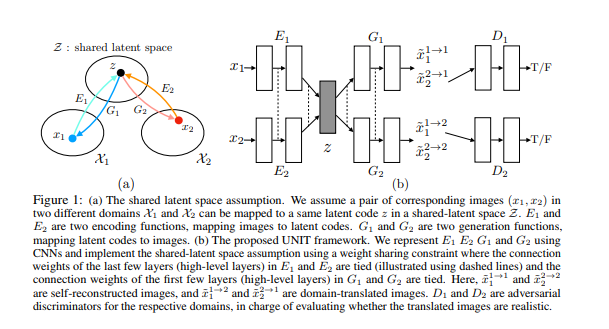
\includegraphics[width=.9\linewidth]{./img/uiit_abst.PNG}
\caption{論文より引用}
\end{figure}

\item \href{https://arxiv.org/abs/1703.10593}{CycleGAN}\\

誰でも知っているので挙げました。解説は\href{https://qiita.com/hikaru-light/items/98d06b21b4f3e2bb6ca4}{このあたり}で見てください。\\
\end{itemize}

\subsection{画像の色付け}
\label{sec:org6163ef7}
\begin{itemize}
\item \href{http://iizuka.cs.tsukuba.ac.jp/projects/colorization/ja/}{Let there be Color!}\\

グレースケール画像 から カラー画像を作るための手法です。早稲田大学の出したグレースケール画像の自動着彩に関する論文。大域・中域・少域特徴を得るためのネットワーク+色付けのネットワークの4つのネットワークをまとめ、彩色画像を作り、それを元のグレースケール画像と組み合わせることでカラー画像を生成します。テレビなんかでも大きく取り上げられたモデルらしいです。大域的・局所的みたいな文言と、最近出てきた \href{https://qiita.com/koshian2/items/0e40a5930f1aa63a66b9}{OctConv のモデル} がなんとなく発想が似ている気がしたのでピックアップしました。\\

\item \href{https://richzhang.github.io/ideepcolor/}{Real-Time User-Guided Image Colorization with Learned Deep Priors}\\

グレースケール画像 から カラー画像を作るための手法です。着彩画像に修正が出来ることなど、ほぼほぼ style2paint と同じ仕様になっていますが、こちらは大体の位置に色を置く(塗るではない)することで着彩を行い、スケッチではなくグレースケール画像を入力に用います。かなり良い精度が出ており、これ、 \textbf{グリザイユ画法} で使えるんじゃね?と一人思っています。(数年くらい前から日本の一部コミュニティではグリザイユ画法が流行っているという \textbf{学術的に価値のない} モチベーションですね)ちなみに GANs のアイデアは使っているのに GANs の損失関数を使わないという面白い内容になっています。GANs を使わないでスタイル変換する論文をこの GANs 時代に提案してくるか…と関心しました。簡単な解説は \href{https://github.com/DwangoMediaVillage/paper\_readings/issues/8}{ここ} を読むと良いと思います。そして恐らくこれが最も本論文である style2paint に影響を与えていると思います(具体的には U-net 周りのアーキテクチャがかなり似通っています)。( \texttt{ただ見た目の精度が尋常じゃないのに評価手法がPSNRなのが結構気になります} )\\

またこの論文では、ユーザの入力に対するシミュレーションも行っており、実際 style2paint でも用いられており、この手のデータ収集に関して非常に参考になるものですので、 \textbf{一読するべき} でしょう(4ページの Simulating User Interactions. の部分です)\\

\begin{figure}[htbp]
\centering
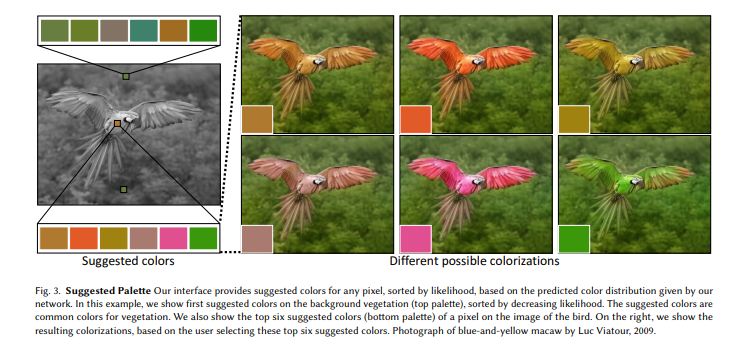
\includegraphics[width=.9\linewidth]{./img/rtugi_abst.PNG}
\caption{論文より引用}
\end{figure}
\end{itemize}

\section{モデル概要}
\label{sec:org00ba3dc}
論文では、提案手法の概要から2段階のステップそれぞれの構成、そして訓練データの作成手法についての説明がなされています。これらをざっくりと消化していきます。特に訓練データの作成・獲得手法については \textbf{pixiv のサーバダウンを狙ってスクレイピングアタック仕掛けている新進気鋭超頭脳AI研究者様} には見ていただきたいものですね。(\sout{界隈や大学の印象悪くなるからやめてくれ})\\

\subsection{OverView}
\label{sec:orgffcb23d}
2段階なフレームワークである本手法は、 \textbf{drafting stage} と \textbf{refinement stage} という名前で2つを区別しています。入力のスケッチと最初に与えられるユーザの指示を元に色の構成を決めて、ぱっと色付けをすることが drafting stage での目標になります。そして refinement stage では drafting stage での drafting stage で得られた画像について不正確な色の領域を識別して、追加のユーザからの指示群を元に改良します。これら2つの stage に対するモデルは別々に訓練されており、実際に検証を行う際に初めて接続され最終出力までを得ることが出来ます。以下の図 Fig. 3 がフレームワークの全体図です。この 2段階なフレームワークは複雑な着彩タスクをよりシンプルで目標が明確であるサブタスクに分割したことで、結果的にスケッチと着彩までの距離を狭めます。さらに学習が容易になり、着彩結果の品質が向上します。一方既存の1段階な着彩手法では学習が困難であるために、不自然な着彩に対する修正を行うことが出来ません。\\

訓練に際して \textbf{着彩済みなデータセット} として目をつけたものは \href{https://www.gwern.net/Danbooru2018}{Danbooru database} でした。これに対するスケッチの獲得は、PaintsChainer による線画抽出システムを用いました。またユーザからの入力(指示)をシミュレートするには、\href{https://arxiv.org/pdf/1705.02999.pdf}{Real-Time User-Guided Image Colorization with LearnedDeep Priors.} に用いられている手法を用いました。drafting と refinement 両方で用いられている本質的な手法は、 \textbf{GANs} です。Fig. 4 をみると、stacking layer と layer のサイズ、layer 間の接続方式についてわかると思います。訓練時にはおおよそ Adam Optimizerを用いています(where \(\beta_1 = 0.9, \beta_2 = 0.99, lr=1e-5\))。訓練に用いた GPU は Tesla P100 で、バッチサイズは 16 でした(バッチサイズを上げると学習率を下げずに訓練がうまく行く、という論文を google が出していたはずなので、より強いGPU使って上げてみたいですね。)トレーニングのサンプルデータは、元画像から \(224 \times 224\) のサイズのパッチにトリミングされます。とはいえ提案手法のモデルは \href{https://esslab.jp/\~ess/ja/research/sketch/}{Fully Convolutional Network} で構成されているので、本フレームワークの検証段階では \textbf{任意の入力サイズをサポートできる} ようになっています。\\

\begin{figure}[htbp]
\centering
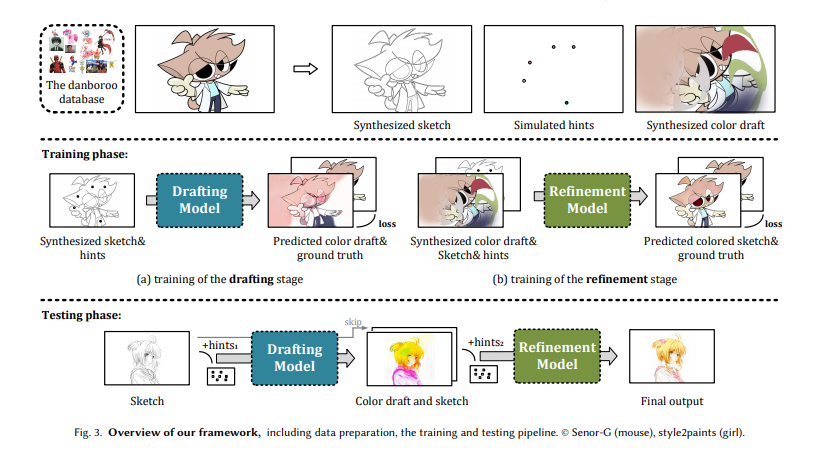
\includegraphics[width=.9\linewidth]{./img/s2p_fig3.PNG}
\caption{Fig.3 論文より引用}
\end{figure}

\begin{figure}[htbp]
\centering
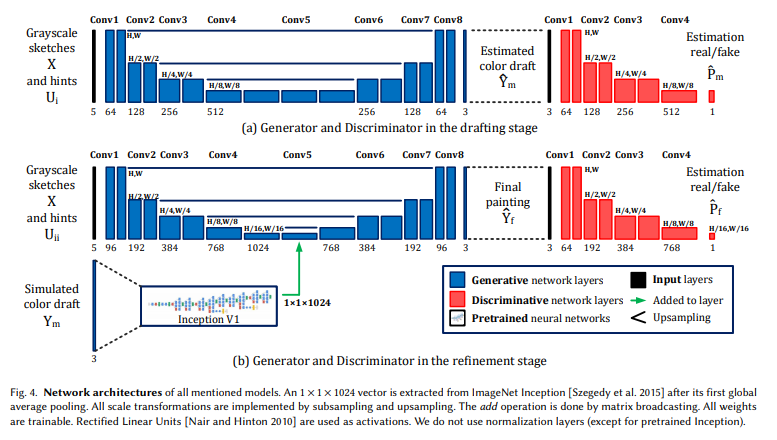
\includegraphics[width=.9\linewidth]{./img/s2p_fig4.PNG}
\caption{Fig.4 論文より引用}
\end{figure}
\subsection{drafting stage}
\label{sec:orgcf8c0e5}
この stage では入力データであるスケッチから大まかな全体の色構成を決定するという目的で学習されます。高品質な画像を求めているわけではなく、色の多様性を保証できるだけ、ユーザの指示に基づいた色を積極的に散らすことが出来る必要があります。このためにスケッチ \(x\) と \(u_i\) から大まかな画像 \(\hat{y}_m\) を予測するネットワーク network G を提案しています。これの概要は Fig.4 (a)にあります。この大まかながぞうのせいせいについては PaintsChainer など他手法が存在していますが、これらは技術的詳細が明らかにされていません。しかし実験の結果、本手法はそれらと同等以上の性能(state-of-art な性能)が得られることがわかりました。\\

スケッチ \(x\) とユーザの指示 \(u_i\) を入力に、 \(G(x, u_i)\) で表される FFN (feed-forward network) で 予測画像 \(\hat{y}_m\) を出力します。最適化のための目的関数は次の式 (1) になります(概形は \textbf{1ノルム} と \textbf{色彩多様性確保のための補正項} 、そして \textbf{GANs} ですね)。\\

\begin{eqnarray}
  arg \min_{G} \max_{D} \mathbb{E}_{x, y_i, y_f \sim P_{data}(x, u_i, y_f)} [&& \|y_f - G(x, u_i)\|_{1} + \alpha L(G(x, u_i))\nonumber  \\ && - \lambda log(D(y_f)) - \lambda log(1 - D(G(x, u_i)))] \\
where && \nonumber \\
L(x) &=& - \Sigma^{3}_{c=1} \cfrac{1}{m} \Sigma^{m}_{i=1}(x_{c, i} - \cfrac{1}{m}\Sigma^{m}_{i=1}x_{c, i})^2 \\
x_{c, i} &=& the\ i-th\ element\ on\ the\ c-th\ cannel \nonumber \\
m &=& image\ width\ \times \ height \nonumber
\end{eqnarray}

損失関数 L では生成される \textbf{色彩のRGB空間における分散を高める効果} を担っており、これによってより \textbf{彩度の高い色をもった} 画像が生成できるようになります。\\

\subsection{refinement stage}
\label{sec:org1dfdfe1}
drafting stage によって得られた画像はまだ色間違いや不自然な部分(英語でこれは artifact と言われます)があるため、実用的ではありません。これを修正するために、修正箇所の領域を特定し、それを修正します。このために本フレームワークではユーザから修正箇所の指摘を受けるという仕組みを取っており、その意図を汲み取り制御することが必要になります。これを他制するために、問題点のある色領域を特定・修正するための別の深層学習モデルを提案しました。このモデルはユーザの指示を受け取り、それに従って色間違いや不自然な部分が修正されます。\\

ところがこのような訓練データを作成することは難しいです。選択肢としては神絵師を札束で殴りつけて draft 画像を修正された画像にしてもらうことですが、これは金も時間もやっべえかかります。またそれによってコンテンツの多様性を確保することも難しいでしょう(神絵師を大量に雇えば良いでしょうが以下略)。あるいは drafting stage から画像を大量に生成してそれを用いるという手法が考えられますが、これを行うと、特定の drafting 画像 に対して過剰適合してしまう可能性があり汎化性能を失う可能性があります。また drafting stage の結果を用いるということはせっかく \textbf{意図的に2つのタスクに分けた} ものをまとめて訓練してしまっていることになることと同義になるので、望ましいものとは思えません。実際に分離したほうがうまく行くことは、本手法の結果を見ればわかります(実際に drafting stage の画像を用いた refinement stage の学習は提案手法に比べ悪い結果が出ています)。\\

上記の手法の代わりに本手法では、\{color draft, refined painting\} の画像ペアを用いた \textbf{データセットを大量に自動合成するための手法} を用いました。この合成手法によって、refinement stage のモデルの汎化性能を上げるために役立ち、モデルが異なる種類の不自然な部分を修正することが出来るようになりました。この自動合成手法では、まず draft 画像の潜在的な不自然な箇所の特徴について実際に得られた draft 画像を観察することから始まります。結果として、draft 画像の不自然な箇所はおおよそ以下のような特徴を持っていました。\\

\begin{itemize}
\item 色の間違い\\

青い太陽とか、緑な人の顔とかその手の色の間違いです。\\

\item 色の染み出し\\

塗りつぶしに失敗した感じです。例えば顔の肌色が背景にまで染み出してしまったことなどが挙げられます。\\

\item ぼやけと歪み\\

低い彩度で水彩塗りがぼやけてしまっているとか、一部の領域が変な質感がかかってしまっているとかしました。\\
\end{itemize}

以降ではこの3点に従うような画像を生成するための手法を説明します。\\

\subsubsection{ランダムな領域切り出しと貼り付け}
\label{sec:org17759fe}
色の間違いをシミュレートするために、カラー画像からランダムに長方形のパッチを切り出します。パッチのサイズは \(64\times 64 \sim 256 \times 256\) の範囲内で、これは一様分布からサンプリングされます。また色の間違いのランダム性と多様性を確保するために、不規則な形状のパッチを得ることができる領域提案法(region proposal methods)を用います。領域は入力画像のエッジマップに基づいて抽出されます。まず、ガウスぼかしをかけた画像と元の画像の差を求め、結果をクリッピングすることでシャープでクリーンなエッジマップを得ます。次に取得したエッジマップを平均値に基づいたしきい値に従って2値化エッジとして再抽出します。最後に不規則な形状のパッチを抽出するための色領域マスクを得るために \href{https://arxiv.org/pdf/1706.06918.pdf}{Trapped-ball segmentation} を実装しました。(\href{https://github.com/pfnet/PaintsChainer/issues/127}{Trapped-ball Segmentationについての議論})\\

これらの2つの方法を組み合わせて、全部で10,000 の異なる画像を抽出します。色の誤りをシミュレートするために、これらのパーツをランダムに回転させて絵の上に重ねて貼り付けます。\\

つまり簡単に言うと、いい感じに学習データからパーツを持ってきて、画像 \(y\) に対して適当に貼り付けることで合成画像 \(y'\) を得ます。\\

\subsubsection{ランダムな変形}
\label{sec:orgcaa4355}
変形を行うことで、ぼやけと歪みをシミュレートします。まず \([0, 0.1^2]\) 以内の正規分布から得られる乱数 \(\theta_{mn}\) を値に持つ \(2\times 3\) 行列 \(T_{\theta}(G)\) を生成します。次に \href{https://papers.nips.cc/paper/5854-spatial-transformer-networks.pdf}{Spatial Transform Layer} (STL) (\href{https://qiita.com/nkato\_/items/125bd2e7c0af582aa32e}{解説})を用いて画像を変形します(STLはどっちかっていうと正規化の手法なんですが、これはとてもユニークな発想ですね、多分)。この変形によって、局所パターンをぼかすことが出来るのと同時に、全体的なノイズ付加ができます。この場合のノイズとは恐らく特徴がボケる、という意味で、画像がぼやける、という意味とはニュアンスが違います。\\

\subsubsection{ランダムな色のスプレー}
\label{sec:orgbeb6123}
画像の上にランダムな色をスプレーすることで、色の染み出しをシミュレートします。まず画像内からランダムな色を取り出します。次にいくつかのランダムな線形のパスに従ってランダムに決められた幅 \(r \sim uniformly\ distribution \in [64, 128]\) でスプレーします。スプレーの形状は、色の染み出しに似た形状のものを選択しています。\\

\begin{figure}[htbp]
\centering
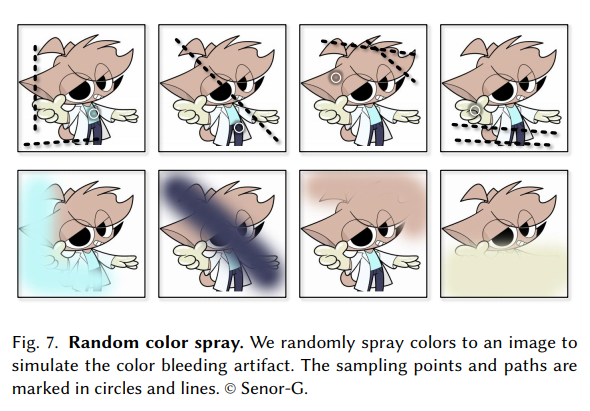
\includegraphics[width=.9\linewidth]{./img/s2p_fig7.PNG}
\caption{Fig.7 論文より引用}
\end{figure}
\subsubsection{モデルの最適化}
\label{sec:org6cac781}
上記の3つの方法を同時に適用することで、draft 画像 \(y_m\) を合成します。スケッチ \(x\) 、 ユーザの指示 \(u_{ii}\) 、 元の画像 \(y_f\)   に対して以下の目的関数を使い学習を行います(\(\lambda = 0.01\))。前の項が GANs のそれで、後の項は1ノルム(MAE, mean absolute error)ですね。 \(y_m\) に関する Encoder の初期の重みとして、 ImageNet の inception V1 を与えました。\\

\begin{eqnarray}
arg \min_{G} \max_{D} \mathbb{E}_{x, u_{ii}, y_m, y_f \sim P_{data}(x, u_{ii}, y_m, y_f)} [-\lambda log(D(y_f)) - \lambda log (1 - D(G(x, u_{ii}, y_m))) + \|y_f - G(x, u_{ii}, y_m)\|_{1}]
\end{eqnarray}

\section{評価}
\label{sec:org00a5089}
性能評価を行うために、まずテストデータセットを用意する必要がありました。このデータセットはインターネットより収集した様々な絵師からの 53 のスケッチで構成されています。スケッチの内容は、人のキャラクタ、動物、植物、風景など多岐にわたります。テストデータセットが学習データに含まれないことを確かにするために、すべてのテストデータを学習データと比較し、それぞれのテストデータに近い画像を上位3つずつ学習データから排除しました。尚画像の近さを測る指標は MSE(Mean Square Error) です。\\

以降の部分は一部を省略しています。論文中の Figure を引用しすぎると翻訳権周りで揉めそうなので、ここでは簡潔にまとめたもので済ませています。概要はすべてまとめられたと思いますが、詳細は元論文を参照してください。\\

\subsection{ユーザインターフェース}
\label{sec:org71dda08}
より便利な着彩環境を構築するために、Fig. 2 のようにユーザが2段階の着彩処理を行うことを支援できるようなユーザインターフェースを設計しました。ユーザインターフェースには 3 つのキャンバスがあり、ツールバー、カラーパレット、そして最終結果のためのものとなっています。先行研究とは異なり、本手法は2段階の結果をそれぞれ別に示して、両方の段階に対するユーザからの指示を受け入れられるようにしました。実験の結果、両方に指示を受けられるようにしたことで、ユーザの着彩処理を高速化させることが出来るとわかりました。\\

\subsection{見た目の比較}
\label{sec:orgd3d4a6e}
まず最初の評価実験として、本手法と他手法との結果の差を視覚的に比較します。いくつかの手法はユーザから \textbf{線} を用いた指示に従って調整を行うが、他の手法では \textbf{点} を用いた指示に従って調整が行われる仕組みになっているので、我々は手動で線を用いた着彩の指示から手動でサンプリングを行ってそれぞれの手法のための適切な \textbf{点} の指示を作成しました。公正な比較を行うために、同一の指示マップが両方の段階で与えられています。異なる指示マップを用いると、結果の品質がより良くなるということに注意してください。\\

\subsubsection{色伝搬手法}
\label{sec:org28b2070}
色伝搬手法からの比較対象として、 \href{https://dcgi.fel.cvut.cz/home/sykorad/Sykora09-EG.pdf}{Lazy Brush} を取り上げました。 Fig.8 を見ればわかるように質感や陰影なしの平坦な色付けしか出来ていないことがわかります。また色滲みの問題も申告で、例えば蛇の塗りつぶしに至ってはその殆どが真っ黒になっていますし、髪飾りも同様な問題を抱えていることがわかります。しかし提案手法では、 Lazy Brush と比較して、質感や陰影を表現できている他、ユーザからの指示によって適切な色伝搬が出来ているとわかります。\\

\subsubsection{機械学習ベースのスケッチの着彩手法}
\label{sec:org2b8982f}
機械学習ベースの着彩手法として、Comicolorization と PaintChainer (V1 \textasciitilde{} V3) を取り上げました。しかし、\href{https://nico-opendata.jp/ja/casestudy/comicolorization/index.html}{Comicolorization}  はスケッチからの色付けに対応した手法ではないので、こちらではスケッチからおおよそグレースケールの着彩が施されています。PaintChainer はどのバージョンでも色滲みの問題があることがわかります。例えば蛇の画像や髪飾りは明らかに色が漏れていることがわかります。その上 V1 に関しては、水彩なぼやけを起こしていることがわかります。この特徴は特に彩度の低い色で見られるようです。V2 では色がよりはっきりとしてきていますが、質感生成の部分で難があるように思われます。例えば蛇の画像ではV1に比べて質感が薄いように見えます。少女の髪の塗りについては、細かい質感や陰影なしにほぼ無地に塗りつぶされていることがわかります。V3 では、質感や陰影の表現はある程度向上していますが、細部や線画歪んでしまっています。また髪飾りのようないくつかの細かい領域に関しては、彩度の高い色や歪んだ色で色付けされています。\\

これに対して提案手法では、ユーザの指示に従って適切な領域に対して着彩を行えている他、ハイライトや乗算のようなレイヤー効果を出すことが出来ていると考えられます(レイヤー云々は絵を描かない人からはなんのこっちゃと思いますが、そういう分野なので諦めてください)。髪の毛や服は鮮やかな色でかつ滑らかなハイライトや影が表現できていることがわかります。蛇については先行研究で、まだらな質感を表現することに難航していましたが、提案手法ではうまく表現することが出来ていると思われます。また refinement stage で、PaintChainerが抱えていた色にじみの問題は解決していると言えます。\\

\begin{figure}[htbp]
\centering
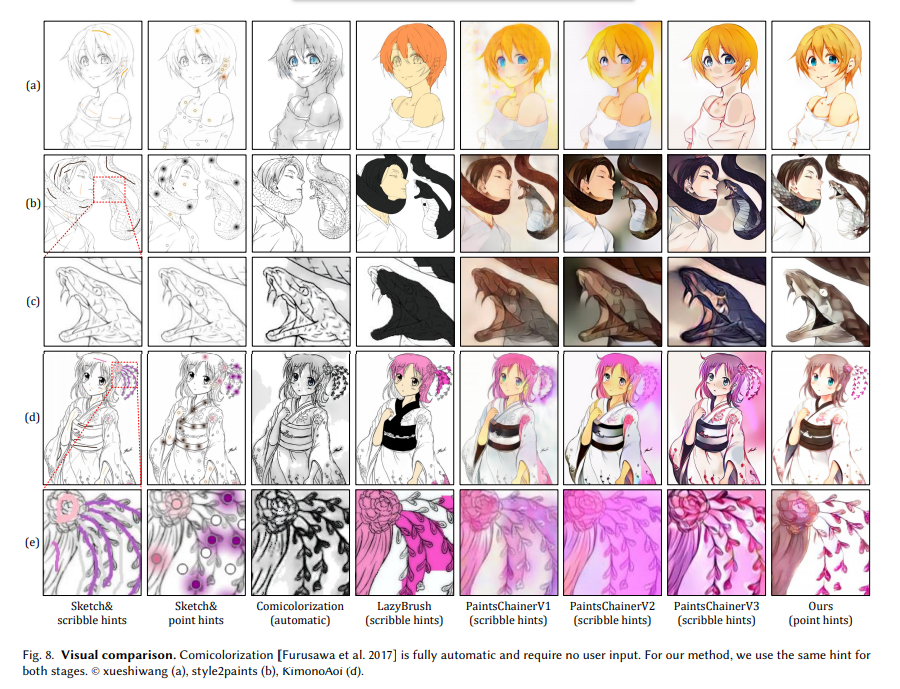
\includegraphics[width=.9\linewidth]{./img/s2p_fig8.PNG}
\caption{Fig. 8 論文より引用}
\end{figure}

また自動着彩、つまりユーザからの指示無しで着祭を行った場合の性能差について比較を行いました。これはユーザが着彩を行う際に何らかのインスピレーションを得たい場合などでの利用が想定されています(論文中 Fig. 9 参照)。PaintChainer V2, V3と、提案手法の自動着彩の性能を比較すると、PaintChainerでは Fig. 8 と同様に色にじみの問題が出ています。またユーザからの指示がないことで、誤った色や色が不自然に混ざってしまっている場面が見られます。提案手法ではこの状態から refinement stage に移ることが出来るため、このような不自然さを修正することが容易であると言えます。\\

\subsubsection{画像スタイルの操作}
\label{sec:org458647a}
ここで用いる画像のスタイル操作、とは参照画像を元にスケッチに着彩を行うという意味です。我々の提案手法と、\href{https://www.cv-foundation.org/openaccess/content\_cvpr\_2016/papers/Gatys\_Image\_Style\_Transfer\_CVPR\_2016\_paper.pdf}{Image Style Transfer Using Convolutional Neural Networks} , \href{https://arxiv.org/pdf/1705.01088.pdf}{Visual attribute transfer through deep image analogy} , \href{https://arxiv.org/pdf/1706.03319.pdf}{Style Transfer for Anime Sketches with Enhanced Residual U-net and Auxiliary Classifier GAN} , \href{https://nico-opendata.jp/ja/casestudy/comicolorization/index.html}{Comicolorization} の4つを用いて比較実験を行いました。結果としてどれも提案手法に比べて、不自然な色を用いていたり、色にじみを起こしてしまっていることがわかりました。また提案手法では比較手法に比べて服の着彩がうまく行くことがわかりました。結果として言えることは、提案手法が半自動的な着彩で、参照画像すべての色を反映するわけではないものの、比較手法に比べて高品質な画像を生成することが出来るということです。\\

\href{https://phillipi.github.io/pix2pix/}{Pix2Pix} のような画像から画像のスタイル変換を用いても勿論スケッチから画像を着彩することが出来ます。比較対象として \href{https://phillipi.github.io/pix2pix/}{Pix2Pix} を取り上げ実験しました。しかし Pix2Pix では低い彩度の画像しか生成できず、画像が滲んでしまいました(Fig. 13 参照)。\\

また\href{https://arxiv.org/pdf/1705.02999.pdf}{Real-Time User-Guided Image Colorization with LearnedDeep Priors.} を用いた比較実験を行いましたが、こちらは現実の写真よりの画像生成するためのシステムであり、スケッチからイラストのような画像の生成、というタスクにはうまく転用できませんでした(Fig. 13 参照)。具体的には、色の間違いや色に地味が献茶に現れてしまっている点が問題として挙げられます。\\

また他手法の比較とは別に、本手法がどのようなスケッチに有効であるのかを調べるために、男性のキャラクタ、女性のキャラクタ、鳥、風景などの着彩を行う実験を行い、モデルの堅牢性を確かめました。結果、提案手法はさまざまな主題や描画スタイルにかかわらずしっかりとした着彩が出来ていることがわかりました(Fig. 10, Fig. 24 を参照)。\\

また特にアジアの絵師に多く見られる、多様な着彩手法についての実験を行いました。繊細な質感や、細かい目のディティール付けなど、絵師によって様々な着彩スタイルがあり、一部の絵師はそれをスケッチの上でも表現することがあります。これは推論を困難にする可能性がありますし、異なる描画スタイルを学習することは、質感やグラデーションを生成することを難しくしてしまう可能性があります。実際 Fig. 11 では比較手法が目の色を表現することが出来ず、詳細な描画領域についてテクスチャを生成することが出来ていないことがわかります。提案手法がこれらの問題に対して堅牢であることの説明に、2段階のフレームワークというデザインにしたことを挙げることが出来ます。つまり複雑な着彩を2つの比較的簡単なタスクに分類したことで、着彩の複雑さを効果的に軽減できたということです。もっと言うならば、refinement stage で質感や陰影の表現を学習することに集中できたことがこの結果を産んだと言えます。また refinement stage は繰り返し修正する機会が得られるので、複雑な描画を確実に処理することが出来ます。\\
\begin{figure}[htbp]
\centering
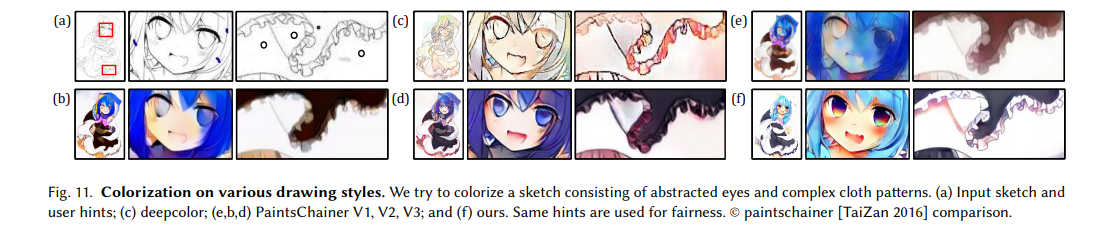
\includegraphics[width=.9\linewidth]{./img/s2p_fig11.PNG}
\caption{Fig.11 論文より引用}
\end{figure}

\subsection{ユーザ実験}
\label{sec:orgc71c844}
提案手法の定量的な評価を得るために、ユーザ実験を行いました。ユーザエクスペリエンスと満足度を評価するために、10人の参加者を募って、作成したGUIソフトを用いてインタラクティブな着彩を行いました。比較対象は PaintsChainer ファミリーで、ランダムに選択された5つのスケッチのセットを着彩しました。参加者はどのようにも指示を行うことが出来ます。また参加者ごとにかかった着彩時間を記録しました。\\

実験後、Fig. 14 に示されるような多次元的な調査を行いました。尚スコアは [0, 1] で正規化されます。また異なる手法間での有意性を検証するために paired student's の T検定 を行いました。結果を Table. 1 に示しました。\\

多次元的な調査に用いた指標は、\\

\begin{itemize}
\item Timing:\\

着彩時間を記録して正規化を施しました。\\

\item User experience:\\

参加者に着彩中にユーザエクスペリエンスを評価してもらいました。\\

\item Regional obedience:\\

参加者にユーザの指示が着際した領域を正確に認識できているのかを評価してもらいました。複数の着彩指示が行われると、モデルはこれに応じて着彩する領域を区別して茶臭いしなければなりません。この評価はまた、モデルが色にじみや色の混合に関する問題をどの程度回避できているのかを暗黙的に評価しています。\\

\item Color obedience:\\

これはモデルがユーザの指示の色域と色調に正確に従うことが出来ているのかを評価します。つまり参加者が赤で塗るように支持すれば、紫などの色ではなく、赤で塗られることを期待しています。\\

\item Visual quality:\\

参加者によって自分が着彩を行って出来た絵を評価してもらいました。なお得点をつける指標として、サンプルの別の絵を見せました。\\
\end{itemize}

統計の結果視覚的な品質や鮮やかさについて、提案手法はPaintsChainerよりも優れているというユーザからの評価が得られたことがわかりました。さらに提案手法では色にじみを抑えれるということがわかりました。つまりユーザの意図を反映した着彩が出来ていることが言えるでしょう。欠点としては提案手法が比較手法と比較して絵の生成に時間がかかってしまうという点です。これは正確な着彩を行うことが出来るという有効性を逆に示せたのではないかと提案者は考えているそうです。実際に、提案手法はユーザの意思を反映して細かいディティールを凝ることが出来るので、参加者は満足できるまで着祭を微調整し続ける傾向がありました。しかし比較手法については細部の着彩についてはあまり効果的ではないため、参加者は早々に諦めてしまう傾向がありました。例えば比較手法では、スケッチの境界を辿った着彩が難しいという問題がありましたが、提案手法ではユーザの指示に従ってそれらを正確に色付けすることが出来ました(Fig. 16 参照)。\\

また Regional obedience についてより深く比較実験を行うために、Lazy Brush を加えた別の比較実験を行いました。実験概要は、Lazy Brush と PaintsChainer と提案手法で、着彩を行ったものについて、スケッチに意味づけられている領域を反映して着彩することが出来ているかを順位付けるというものです。結果として提案手法は平均で 1.22 という最高順位を達成しました。\\

\begin{figure}[htbp]
\centering
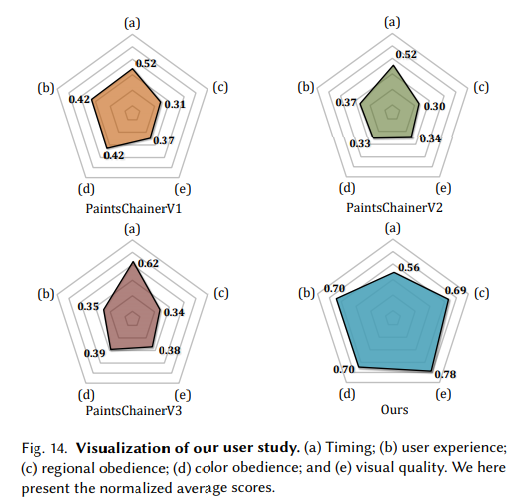
\includegraphics[width=.9\linewidth]{./img/s2p_fig14.PNG}
\caption{Fig. 14 論文より引用}
\end{figure}

\subsection{Discussions and Limitation}
\label{sec:orgfc35280}
To be Continued\ldots{}\\

\section{感想}
\label{sec:orge1eabfc}
僕はあんまり画像系の研究はしていないんですが、この論文はとても読みやすい部類であったと思います。最近読んだ \href{https://arxiv.org/abs/1904.09571}{TransGaGa} の技術を組み合わせるとか \href{https://arxiv.org/abs/1807.03039}{Glow} や U-Net を参考に Fully Connected Network の構築手法をアップデートする(特に refinement stage の ユーザの指示と画像の組み合わせ部分を TransGaGa の CVAE 項みたいにしてみたら面白そうですね)とか、Refinement Stage を強化学習の分野に持ち込んでみるとか、自動画像生成の部分をもっと詰めてみるとか、色々研究していみたいテーマが見える面白い分野だなぁと思いました。(小並感)\\

ところでこの論文を読む限り End-to-End 学習には難がありそうなイメージになっているんですが、最近のトレンド的にどうなんでしょう。\\

最後にこの論文の著者についてです。この著者、物凄いリサーチ力を持っているらしく、先行研究のの実装なんかに積極的に issue を立てて質問に行く(しかも的外れではなくまっとうな質問を!)スタイルはとても尊敬できるなぁと思いました。閉鎖空間で学年やらポストやらで上下関係するスタイルとは違って学問といった雰囲気がしてとても好感が持てます。\\

この後は時間があれば、\href{https://arxiv.org/pdf/1706.03319.pdf}{Style Transfer for Anime Sketches with Enhanced Residual U-net and Auxiliary Classifier GAN} と \href{https://arxiv.org/pdf/1705.02999.pdf}{Real-Time User-Guided Image Colorization with LearnedDeep Priors.} を読もうかなと思っていたり思っていなかったり(\sout{趣味でやっているので、自分の研究時間との兼ね合いが大変})\\

追伸・セルシスさん とか Pixiv さんとか PFN さんとかで研究してくれないかなぁ(チラッチラッ)\\
\end{document}
